%!TEX root =./main.tex
% arara: pdflatex
% arara: makeglossaries
% arara: biber 
% arara: pdflatex while changed('bbl') || changed('gls') || found('log', 'Please rerun') || found('log', 'Label(s) may have changed')

%%**************************************************************
%%
%% DHBW Heidenheim - Template for Bachelor Thesis
%%
%% Bevor usisng this template please have a look at the REAMDME.md file
%%
%%**************************************************************

%!TEX root =../main.tex

% show warning for old LaTeX syntax
\RequirePackage[l2tabu, orthodox]{nag}

\documentclass[
    pdftex,
    oneside,
    12pt,			    % fontsize
    parskip=half,		    % Space (in lines) between paragraphs
    headheight = 20pt,    % Header hight
    headsepline,		    % Line after header
    footheight = 16pt,	    % Footer height
    footsepline,		    % Line before footer
    abstract=true,		    % Abstract headline
    DIV=calc,		    % Calculate print space
    BCOR=8mm,		    % BCOR settings (Bindekorrektur)
    headinclude=false,   % Exclude header from print space
    footinclude=false,	    % Exclude footer from print space
    listof=totoc,		    % Show List of Figures/Tables in Contents
    toc=bibliography,	    % Show Bibliography in Contents
    % appendixprefix = true
]{scrreprt}	                     % Koma-Script report-class, long document: scrreprt, short document: scrbook

\usepackage{xstring}
\usepackage[utf8]{inputenc}
\usepackage[T1]{fontenc}

\usepackage{pifont}

% iflang command definition
\newcommand{\iflang}[2]{%
    \IfStrEq{\documentLanguage}{#1}{#2}{}%
}

% ifDocType comand definition
\newcommand{\ifDocType}[3]{%
    \IfStrEq{\documentType}{#1}{#2}{#3}%
}

% ifMultipleAuthors definition
\newcommand{\ifMultipleAuthors}[2]{%
    \IfStrEq{\multipleAuthors}{true}{#1}{#2}%
}

% ifSpecialDocument definition
\newcommand{\ifSpecialDocument}[2]{\IfStrEqCase{\documentType}{%
        {T2_1000}{#2\ignorespaces}%
            {T2000}{#2\ignorespaces}%
            {T3100}{#2\ignorespaces}%
            {T3300}{#2\ignorespaces}%
    }[#1\ignorespaces]%
}

% setAiNote Command
\newif\ifshowAiNote
\newcommand{\setAiNote}[1]{%
  \csname showAiNote#1\endcsname%
}

% setGenderNote Command
\newif\ifshowGenderNote
\newcommand{\setGenderNote}[1]{%
  \csname showGenderNote#1\endcsname%
}

% setGlossary Command
\newif\ifshowGlossary
\newcommand{\setGlossary}[1]{%
  \csname showGlossary#1\endcsname%
}

% Include main settings
%!TEX root = ../main.tex

%% Zusätzliche Pakete (Tabellen mit Linien nach booktabs)
\usepackage{booktabs}
% Flattersatz-Spalte für tabularx (verhindert gesperrte Wörter in schmalen Spalten)
\usepackage{array}
\newcolumntype{Y}{>{\raggedright\arraybackslash}X}
% Architekturbild direkt in LaTeX (keine Rastergrafik)
\usepackage{tikz}
\usetikzlibrary{positioning,arrows.meta,fit}

%% Citation Styles
% https://de.overleaf.com/learn/latex/Biblatex_citation_styles
% recommended: for Electrical Engineering/Computer Science: IEEE
\newcommand{\quoteStyle}{ieee}

%% Fonts
%% palatino, goudysans, lmodern or libertine
\newcommand{\documentFont}{lmodern}

%% Margin
\newcommand{\margin}{2.5cm}

%% Space between chapter headline and top of page
\newcommand{\chapterMargin}{20pt}

%% Table settings
% Column spacing
\newcommand{\tableColumnMargin}{10pt}
%Line spacing
\newcommand{\tableRowMargin}{1.5}

%% Color settings
\newcommand{\defineColors}{%
	\definecolor{LinkColor}{HTML}{\linkColor}
	\definecolor{ListingBackground}{HTML}{F8F8F8}
}

%% Syntax Highlighting (Listings)
\newcommand{\listingsettings}{%
	\lstset{%
		language={},			% default language (keine Syntaxhervorhebung)
		numbers=left,			% position of line numbers (left, right)
		stepnumber=1,			% set number to each line
		numbersep=5pt,			% 5pt between number and source code
		numberstyle=\tiny,		% letter size of numbers
		breaklines=true,		% break lines if necessary (true, false)
		breakautoindent=true,	% indenting after break line (true, false)
		postbreak=\space,		% break line after space
		tabsize=2,				% tabulator size
		basicstyle=\ttfamily\footnotesize, % font style
		columns=fullflexible,	% natürliche Zeichenabstände
		showspaces=false,		% show space (true, false)		
		showstringspaces=false,	% show space in strings (true, false)
		extendedchars=true,		% show all Latin1 characters (true, false)
		captionpos=b,			% sets the caption-position to bottom
		backgroundcolor=\color{ListingBackground}, % source code background
		xleftmargin=10pt,		% margin left
		xrightmargin=5pt,		% margin right
		frame=single,			% border settings
		frameround=ffff,
		rulecolor=\color{darkgray},	% border color
		fillcolor=\color{ListingBackground},
		aboveskip=20pt,
		keywordstyle=\color[rgb]{0.133,0.133,0.6},
		commentstyle=\color[rgb]{0.133,0.545,0.133},
		stringstyle=\color[rgb]{0.627,0.126,0.941},
		% Umlaute und Sonderzeichen in Listings (pdflatex)
		literate={ä}{{\"a}}1 {ö}{{\"o}}1 {ü}{{\"u}}1 {Ä}{{\"A}}1 {Ö}{{\"O}}1 {Ü}{{\"U}}1 {ß}{{\ss}}1
			{€}{{\texteuro}}1 {³}{{\textthreesuperior}}1 {·}{{\textperiodcentered}}1 {–}{{--}}1
	}
}


% Include document settings
%!TEX root = ../main.tex

%% Document language (en, de)
\newcommand{\documentLanguage}{de}

%% Document type
% T1000 Project Thesis (Semester 1 & 2)
% T2000 Project Thesis (Semester 3 & 4)
% T3100 Seminar Paper (Semester 5 & 6)
% T3300 Bachelor Thesis
% or custom type like 'Hausarbeit'
% Prüfungsleistung laut Aufgabenstellung: "Konzeptentwurf für einen eigenen KI-Agenten-Prototyp"
% (feminin gewählt, damit "meine/dieser ..." in Erklärung und Hinweisen grammatisch passt)
\newcommand{\documentType}{Konzeptarbeit}
\newcommand{\showCompanyLogo}{false}

% Whether to show the ai note at the beginning
% TODO: Text in ads/aiNote.tex an die tatsächliche Nutzung und die Vorgaben der Hochschule anpassen
\setAiNote{true}

% Whether to show the gender note at the beginning
\setGenderNote{true}

% Wether to show a glossary at the end
\setGlossary{false}

\newcommand{\multipleAuthors}{false}
\newcommand{\documentAuthor}{Dennis Gerhardt}
\newcommand{\documentTitle}{LocalLLM: Ein lokaler Agent für private Rechnungen und Verträge}
\newcommand{\documentPeriod}{Oktober -- November 2026}

% TODO: Matrikelnummer und Kurs eintragen
\newcommand{\matriculationNumber}{0000000}

% TODO: Standort, Studiengang und Kurs prüfen
\newcommand{\locationUniversity}{Mosbach}
\newcommand{\department}{Informatik}
\newcommand{\course}{KURS}

\newcommand{\degree}{Bachelor of Science}
% INF2014 - INF2016 (MI):       Bachelor of Science
% INF2014 - INF2016 (IA/IM) :   Bachelor of Engineering
% INF2017 (all):                Bachelor of Science

% A lecture that the document is written for
\newcommand{\lecture}{Agentensysteme: Local Agentic AI}
% Whether to show the lecture on cover
\newcommand{\showLecture}{true}

% TODO: Abgabedatum und -ort prüfen
\newcommand{\releaseDate}{November 2026}
\newcommand{\releaseLocation}{Mosbach}

% Dualer Partner und Betreuer erscheinen bei der Konzeptarbeit nicht auf dem Deckblatt
\newcommand{\companyName}{Dualer Partner}
\newcommand{\companyLocation}{Ort}

\newcommand{\tutor}{--}
% TODO: Dozent der Vorlesung eintragen (steht auf dem Deckblatt)
\newcommand{\evaluator}{Name des Dozenten}

\newcommand{\linkColor}{000000}


% Load language specific Strings
\input{lang/\documentLanguage}

% Load language specific babel package
\iflang{de}{\usepackage[english, ngerman]{babel}}
\iflang{en}{\usepackage[ngerman, english]{babel}}

% Add comment feature
\newcommand{\comment}[1]{\par {\bfseries \color{blue} #1 \par}}




%%%%%%% Package Includes %%%%%%%
\usepackage[margin=\margin, foot=1cm]{geometry}
\usepackage[onehalfspacing]{setspace}
\usepackage{makeidx}
\usepackage[autostyle=true,german=quotes]{csquotes}
\usepackage{enumitem}
\usepackage{graphicx}
\usepackage{pdfpages}
\usepackage{xcolor}
\usepackage{float}
\usepackage{calc}
\usepackage{wrapfig}
\usepackage[perpage, hang, multiple, stable, bottom]{footmisc}
\usepackage{listings}
\usepackage{amsmath}
\usepackage{amssymb}
\usepackage{\documentFont}
\usepackage[%
    pdftitle={\documentTitle},
    pdfauthor={\documentAuthor},
    pdfsubject={\documentType},
    pdfcreator={pdflatex, LaTeX with KOMA-Script},
    pdfpagemode=UseOutlines,       % Show Contents while opening
    pdfdisplaydoctitle=true, 		% Show document title instead of file name
    pdflang={\documentLanguage}, % Document language
]{hyperref}
\usepackage{bookmark}
\usepackage[nonumberlist,toc,acronym,nopostdot]{glossaries}
\usepackage{scrhack}
\usepackage{tabularx}
\usepackage{afterpage}

% Appendix
\usepackage[toc, page, title, titletoc, header]{appendix}
\renewcommand{\appendixname}{\appendixPhrase}
\renewcommand{\appendixtocname}{\appendixPhrase}
\renewcommand{\appendixpagename}{\appendixPhrase}
\renewcommand{\autodot}{}

% Seperate Appendix TOC
\DeclareNewTOC[%
    owner=\jobname,
    listname={\appendixtocPhrase},% title of the appendix ToC
]{atoc}

\makeatletter
\newcommand*\appendixtoc{%
    \renewcommand*{\ext@toc}{atoc}%
    \scr@ifundefinedorrelax{hypersetup}{}{\hypersetup{bookmarkstype=atoc}}%
    \listofatocs
}
\makeatother

% Generate glossary
\makeglossaries{}

% Load colors
\defineColors{}

% Set Titel, Autor and Date
\title{\documentTitle}
\author{\documentAuthor}
\date{\datum}


% PDF link settings
\hypersetup{%
    colorlinks=true,
    linkcolor=LinkColor,
    citecolor=LinkColor,
    filecolor=LinkColor,
    menucolor=LinkColor,
    urlcolor=LinkColor,
    linktocpage=true,
    bookmarksnumbered=true
}

% Captions fontsize
\addtokomafont{caption}{\small}

% Bibliographie settings
\iflang{de}{%
    \usepackage[
        backend=biber,		% recommended. Alternative: bibtex
        bibwarn=true,
        bibencoding=utf8,	         % If.bib file is encoded with utf8, otherwise ascii
        sortlocale=de_DE,
        style=\quoteStyle,
        maxnames=5,
        minnames=4,
        dashed=false
    ]{biblatex}
    \DefineBibliographyStrings{german}{andothers={et\addabbrvspace al\adddot}}
}
\iflang{en}{%
    \usepackage[
        backend=biber,		% recommended. Alternative: bibtex
        bibwarn=true,
        bibencoding=utf8,        % If.bib file is encoded with utf8, otherwise ascii
        sortlocale=en_US,
        style=\quoteStyle,
        maxnames=5,
        minnames=4,
        dashed=false
    ]{biblatex}
}

\setcounter{biburllcpenalty}{7000}
\setcounter{biburlucpenalty}{8000}

% \bibliography{bibliographie.bib}
\addbibresource{bibliographie.bib}

% Hurenkinder und Schusterjungen verhindern
% http://projekte.dante.de/DanteFAQ/Silbentrennung
\clubpenalty = 10000 % schließt Schusterjungen aus (Seitenumbruch nach der ersten Zeile eines neuen Absatzes)
\widowpenalty = 10000 % schließt Hurenkinder aus (die letzte Zeile eines Absatzes steht auf einer neuen Seite)
\displaywidowpenalty=10000

% Graphicspath
\graphicspath{{images/}}

% frequently used programing languages
\lstloadlanguages{PHP,Python,Java,C,C++,bash}

\listingsettings{}
% Rename Listings
\renewcommand\lstlistingname{\listingPhrase}
\renewcommand\lstlistlistingname{\listListingPhrase}
\def\lstlistingautorefname{\authorListingPhrase}

% Spaces in tables
\setlength{\tabcolsep}{\tableColumnMargin}
\renewcommand{\arraystretch}{\tableRowMargin}


%!TEX root = ../main.tex

%
% To create glossary run the following command:
% makeglossaries main.acn && makeglossaries main.glo
%

% Abkürzungen (nur verwendete erscheinen im Abkürzungsverzeichnis)

\newacronym{API}{API}{Application Programming Interface}
\newacronym{BM25}{BM25}{Best Matching 25 (lexikalisches Ranking-Verfahren)}
\newacronym{CPU}{CPU}{Central Processing Unit}
\newacronym{CRAG}{CRAG}{Corrective Retrieval-Augmented Generation}
\newacronym{GPU}{GPU}{Graphics Processing Unit}
\newacronym{JSON}{JSON}{JavaScript Object Notation}
\newacronym{KI}{KI}{Künstliche Intelligenz}
\newacronym{LLM}{LLM}{Large Language Model}
\newacronym{MRR}{MRR}{Mean Reciprocal Rank}
\newacronym{OCR}{OCR}{Optical Character Recognition}
\newacronym{OOM}{OOM}{Out of Memory}
\newacronym{RAG}{RAG}{Retrieval-Augmented Generation}
\newacronym{RRF}{RRF}{Reciprocal Rank Fusion}


\begin{document}

% Cover
\begin{spacing}{1}
    %!TEX root = ../main.tex

\begin{titlepage}

    
\includegraphics[height=2.5cm]{images/cover/logo-dhbw.pdf}
    \IfStrEq{\showCompanyLogo}{true}{
        \hfill
        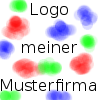
\includegraphics[height=2.5cm]{images/cover/logo-company.png}
    }
    
    \enlargethispage{20mm}
    \begin{center}
        \doublespacing{
            \vspace*{12mm}
            {\LARGE\textbf\documentTitle}
        }\\
        \vspace*{12mm}
        {\large\textbf\documentTypePhrase}\\

        % degre only for bachelor thesis
        \ifDocType{T3300}{
            \vspace*{12mm}
            \degreePhrase\\
            \vspace*{3mm}
            {\textbf\degree}\\
        }

        \IfStrEq{\showLecture}{true}{
            \vspace*{12mm}
            \lecturePhrase\\
            \vspace*{0mm}
            {\textbf\lecture}\\
        }

        \vspace*{12mm}\departmentPhrase\space\department\\
        \vspace*{0mm}\locationUniversityPhrase{} \locationUniversity\\
        \vspace*{12mm}\documentAuthorPhrase\\
        \vspace*{3mm}
        {\large\textbf\documentAuthor}\\
        \vspace*{12mm}\releaseDate\\
        \vfill
        \begin{spacing}{0.8}
            % Eigene Dokumenttypen (z. B. Konzeptarbeit): ohne Dualen Partner und betrieblichen Betreuer
            \ifSpecialDocument{%
                \begin{tabular}{@{}p{0.47\textwidth}p{0.47\textwidth}@{}}
                    \textbf{\documentPeriodPhrase}                     & \documentPeriod               \\
                    \textbf{\matriculationNumberPhrase, \coursePhrase} & \matriculationNumber, \course \\
                    \textbf{Dozent}                                    & \evaluator
                \end{tabular}%
            }{%
                \begin{tabular}{@{}p{0.47\textwidth}p{0.47\textwidth}@{}}
                    \textbf{\documentPeriodPhrase}                     & \documentPeriod                \\
                    \textbf{\matriculationNumberPhrase, \coursePhrase} & \matriculationNumber, \course  \\
                    \textbf{\companyPhrase}                            & \companyName, \companyLocation \\
                    \textbf{\tutorPhrase}                              & \tutor                         \\
                    \textbf{\evaluatorPhrase}                          & \evaluator
                \end{tabular}%
            }
        \end{spacing}
    \end{center}
\end{titlepage}

\end{spacing}
\newpage

\pagenumbering{Roman}

% Restriction notices
% Kein Sperrvermerk: Die Arbeit enthält keine vertraulichen Firmendaten.
% %!TEX root = ../main.tex

\thispagestyle{empty}

\section*{\restrictionNoticesPhrase}

\vspace*{2em}

\iflang{de}{%
  Die vorliegende Arbeit beinhaltet vertrauliche Informationen der Firma {\companyName}.
  Sie ist nur für die Beteiligten am Begutachtungs- und Evaluationsprozess bestimmt.

  Die Weitergabe des Inhalts der Arbeit im Ganzen oder von Teilen daraus an externe Dritte sowie das Anfertigen von Abschriften oder Kopien zu welchem Zweck, in welcher Form und zu welchem Zeitpunkt auch immer, sind grundsätzlich untersagt.

  Ausnahmen bedürfen der schriftlichen Genehmigung der Firma {\companyName}.
  Eine Weitergabe an Mitarbeiter der Hochschule aufgrund fachlicher Belange oder für administrative Zwecke ist von dieser Regelung explizit ausgenommen.
}

%http://www.ib.dhbw-mannheim.de/fileadmin/ms/bwl-ib/Downloads_alt/Leitfaden_31.05.pdf

\iflang{en}{%
  The {\documentTypePhrase} on hand
  \begin{center}{\itshape{} \documentTitle{}\/}\end{center}
  contains internal resp.\ confidential data of {\companyName}. It is intended solely for inspection by the
  assigned examiner, the head of the {\department} department and, if necessary, the Audit
  Committee \locationUniversityPhrase{} {\locationUniversity}. It is strictly forbidden
  \begin{itemize}
    \item to distribute the content of this paper (including data, figures, tables, charts etc.) as a whole or
          in extracts,
    \item to make copies or transcripts of this paper or of parts of it,
    \item to display this paper or make it available in digital, electronic or virtual form.
  \end{itemize}
  Exceptional cases may be considered through permission granted in written form by the author
  and {\companyName}.
}

\vspace{3em}

\releaseLocation, \releaseDate
\vspace{4em}

\rule{6cm}{0.4pt}\\
\documentAuthor

% \newpage

% Declaration
%!TEX root = ../main.tex

\thispagestyle{empty}

\section*{\declarationPhrase}

\vspace*{2em}

\iflang{de}{%
  \ifMultipleAuthors{Wir versichern}{Ich versichere} hiermit, dass \ifMultipleAuthors{wir unsere}{ich meine}
  {\documentTypePhrase} mit dem Thema {\itshape \documentTitle }
  selbstständig verfasst und  keine anderen als die angegebenen Quellen und Hilfsmittel benutzt \ifMultipleAuthors{haben}{habe}.
  \ifMultipleAuthors{Wir versichern}{Ich versichere} zudem, dass die eingereichte elektronische Fassung mit der gedruckten Fassung
  übereinstimmt.
}


\iflang{en}{%
  Hereby \ifMultipleAuthors{we}{I} solemnly declare:
  \begin{enumerate}
    \item that this {\documentTypePhrase}, titled {\itshape \documentTitle } is entirely the product of \ifMultipleAuthors{our}{my}
          own scholarly work, unless otherwise indicated in the text or references, or acknowledged below;
    \item \ifMultipleAuthors{we}{I} have indicated the thoughts adopted directly or indirectly from other sources at the appropriate
          places within the document;
    \item this {\documentTypePhrase} has not been submitted either in whole or part, for a degree at this or
          any other university or institution;
    \item \ifMultipleAuthors{we}{I} have not published this {\documentTypePhrase} in the past;
    \item the printed version is equivalent to the submitted electronic one.
  \end{enumerate}
  \ifMultipleAuthors{We are}{I am} aware that a dishonest declaration will entail legal consequences.
}

\vspace{3em}

\releaseLocation, \releaseDate
\vspace{4em}

\rule{6cm}{0.4pt}\\
\documentAuthor

\newpage

% AI
\ifshowAiNote
    %!TEX root = ../main.tex

\thispagestyle{empty}

\section*{Hinweis auf Nutzung von KI}

\vspace*{2em}

\iflang{de}{%
  Im Rahmen der Erstellung dieser \documentTypePhrase wurden KI-basierte Hilfsmittel \textbf{ausschließlich} zur sprachlichen Überarbeitung (Rechtschreibprüfung, Grammatikkorrektur, stilistische Glättung) verwendet.
  Die inhaltliche Verantwortung sowie die wissenschaftliche Argumentation liegen vollumfänglich bei \documentAuthor.
}


\iflang{en}{%
  In the context of preparing this \documentTypePhrase, AI-based tools were used \textbf{exclusively} for linguistic revision (spelling check, grammar correction, stylistic refinement).
  The responsibility for the content and the scientific argumentation lies entirely with \documentAuthor.
}

\vspace{3em}

% \releaseLocation, \releaseDate
\vspace{4em}

% \rule{6cm}{0.4pt}\\
% \documentAuthor

    \newpage
\else
    % no ai note
\fi

% Gender
\ifshowGenderNote
    %!TEX root = ../main.tex

\thispagestyle{empty}

\section*{Gender-Hinweis}

\vspace*{2em}

\iflang{de}{%
  Zur besseren Lesbarkeit wird in dieser \documentTypePhrase das generische Maskulinum verwendet. Die in dieser \documentTypePhrase verwendeten Personenbezeichnungen beziehen sich – sofern nicht anders kenntlich gemacht – auf alle Geschlechter.
}


\iflang{en}{%
  You don't need this german shit. Just deleate the block with \lstinline[breaklines=false]|%!TEX root = ../main.tex

\thispagestyle{empty}

\section*{Gender-Hinweis}

\vspace*{2em}

\iflang{de}{%
  Zur besseren Lesbarkeit wird in dieser \documentTypePhrase das generische Maskulinum verwendet. Die in dieser \documentTypePhrase verwendeten Personenbezeichnungen beziehen sich – sofern nicht anders kenntlich gemacht – auf alle Geschlechter.
}


\iflang{en}{%
  You don't need this german shit. Just deleate the block with \lstinline[breaklines=false]|%!TEX root = ../main.tex

\thispagestyle{empty}

\section*{Gender-Hinweis}

\vspace*{2em}

\iflang{de}{%
  Zur besseren Lesbarkeit wird in dieser \documentTypePhrase das generische Maskulinum verwendet. Die in dieser \documentTypePhrase verwendeten Personenbezeichnungen beziehen sich – sofern nicht anders kenntlich gemacht – auf alle Geschlechter.
}


\iflang{en}{%
  You don't need this german shit. Just deleate the block with \lstinline[breaklines=false]|\input{ads/genderNote.tex}| in main.tex
}

\vspace{3em}

% \releaseLocation, \releaseDate
\vspace{4em}

% \rule{6cm}{0.4pt}\\
% \documentAuthor
| in main.tex
}

\vspace{3em}

% \releaseLocation, \releaseDate
\vspace{4em}

% \rule{6cm}{0.4pt}\\
% \documentAuthor
| in main.tex
}

\vspace{3em}

% \releaseLocation, \releaseDate
\vspace{4em}

% \rule{6cm}{0.4pt}\\
% \documentAuthor

    \newpage
\else
    % no gender note
\fi

% Abstract
%!TEX root = ../main.tex


\makeatletter
\renewenvironment{abstract}{%
    \thispagestyle{empty}
    \@beginparpenalty\@lowpenalty
    \begin{center}%
        \bfseries \abstractname
        \@endparpenalty\@M
    \end{center}
}%

{\par\vfil\null}
\makeatother

\begin{abstract}
% Abstract in Deutsch
LocalLLM ist ein Agent, der Fragen zu privaten Rechnungen und Verträgen beantwortet. Er läuft vollständig auf einem Laptop mit 16\,GB Arbeitsspeicher und ohne Grafikkarte, damit keine persönlichen Daten den Rechner verlassen. Er liest PDF- und DOCX-Dateien mit ihrer Struktur ein: Tabellenzeilen mit Spaltenkopf, Kapitelpfad, Diagrammbeschreibung und geprüfte Kerndaten. Jede Antwort bekommt nummerierte Quellen. Ich vergleiche zwei Prototypen. P1 zeigt erst die Belege und lässt dann das Modell Werte mit Belegnummer liefern, die Code prüft. P2 ist ein ReAct-Agent, der selbst aus acht Werkzeugen wählt. Getestet wird nicht durch Ausprobieren, sondern mit begründeten Fragen, Sollwerten aus den Dokumenten und versiegelten Testsätzen. Ich nutze drei Kennzahlen: eine eigene Korrektheitsregel sowie Faithfulness und Context Recall aus RAGAS. Ein Reverse Engineering verfolgt eine Frage durch alle Bausteine und zeigt, wo Fehler entstehen. Auf 24 ungesehenen Fragen beantwortet P1 14 richtig, P2 7. Fragen nach Dokumenten, die es nicht gibt, lehnt P1 in drei von vier Fällen richtig ab, weil Code den Bestand prüft. Für P1 ist meist nicht die Suche der Engpass (Context Recall 0,80), sondern das kleine Sprachmodell beim Lesen der Belege; RAGAS-Faithfulness findet dabei unbelegte Aussagen, die eine reine Zahlprüfung übersieht.
\end{abstract}

\begin{otherlanguage}{english}
    \begin{abstract}
    % Abstract in Englisch
    LocalLLM is an agent that answers questions about private invoices and contracts. It runs entirely on a laptop with 16\,GB of RAM and no graphics card, so no personal data leaves the machine. It ingests PDF and DOCX files with their structure: table rows with column headers, section paths, chart descriptions and verified key facts. Every answer carries numbered sources. Two prototypes are compared. P1 shows the evidence first and then lets the model return values with evidence numbers, which code checks. P2 is a ReAct agent that chooses from eight tools itself. Testing does not rely on trying things out but on justified questions, expected values taken from the documents and sealed test sets. Three metrics are used: a rule-based correctness check plus faithfulness and context recall from RAGAS. A reverse-engineering walk-through follows one question through every component and shows where errors arise. On 24 unseen questions P1 answers 14 correctly, P2 7. P1 correctly refuses three of four questions about documents that do not exist, because code checks the inventory. For P1 the bottleneck is mostly not retrieval (context recall 0.80) but the small language model reading the evidence; RAGAS faithfulness catches unsupported claims that a pure number check misses.
\end{abstract}
\end{otherlanguage}

\newpage

% only page number in footer
\pagestyle{plain}

% space bevore chapter headline
\RedeclareSectionCommand[beforeskip=\chapterMargin]{chapter}

% Contents
\begin{spacing}{1.05}
\begingroup

% set subchapter depth
\setcounter{tocdepth}{2}

\tableofcontents
\clearpage
\endgroup

\newpage

% Acronyms
\cleardoublepage
\printglossary[type=acronym, title={\acronymsPhrase}, style=index]

% List of Figures
\cleardoublepage
\listoffigures

%List of Tables
\cleardoublepage
\listoftables

% List of Listings
\cleardoublepage
\lstlistoflistings
\cleardoublepage

\end{spacing}

\pagenumbering{arabic}

\pagestyle{headings}

% Content: Kapitel ohne Seitenumbruch (Umfangsvorgabe 5-8 Seiten)
\begingroup
\RedeclareSectionCommand[style=section, beforeskip=-1.2\baselineskip, afterskip=0.6\baselineskip, font=\Large\bfseries]{chapter}
%!TEX root = ../../../main.tex

\chapter{Problem, Idee und Daten}
\label{chap:problem}

\paragraph{Problem.} Zu Hause sammeln sich Rechnungen und Verträge. Will ich etwas wissen, muss ich die richtige Stelle in der richtigen Datei finden, oft in zwei Dateien (\enquote{Stimmt der Abschlag der Rechnung mit dem Vertrag überein?}). Mein Agent beantwortet solche Fragen über alle Dokumente, belegt jede Aussage mit einer nummerierten Quelle und sagt, wenn nichts belegt ist. Weil die Dokumente IBAN, Adressen und Gesundheitsdaten enthalten, läuft alles lokal auf meinem Laptop (16\,GB RAM, keine Grafikkarte) mit Ollama und ChromaDB.

\paragraph{Fragetypen.} Meine eigenen Fragen fallen in fünf Typen (Tabelle~\ref{tab:fragetypen}). Sie bestimmen die Architektur: Für a und b reicht eine gute Suche, c braucht zwei Dokumente zugleich, d alle Verträge, und e muss der Agent als unbeantwortbar erkennen.

\begin{table}[H]
    \centering\footnotesize\setstretch{1.05}
    \begin{tabularx}{\textwidth}{@{}l Y Y@{}}
        \toprule
        \textbf{Typ} & \textbf{Beispiel} & \textbf{Was der Agent dafür braucht} \\
        \midrule
        a) Wert aus Tabelle & Wie viel Umsatzsteuer weist die LuminaStyle-Rechnung aus? & die richtige Tabellenzeile mit Spaltenkopf \\
        b) Textstelle & Wie lange läuft der Handyvertrag mindestens? & den richtigen Abschnitt im Vertrag \\
        c) Zwei Dokumente & Passt die Vorauszahlung der Wasserabrechnung zum Vertrag? & Rechnung \emph{und} Vertrag, die zusammengehören \\
        d) Liste & Welche Verträge verlängern sich automatisch um ein Jahr? & alle Verträge, Fristen richtig berechnet \\
        e) ohne Beleg & Welche Kündigungsfrist hat mein Handyvertrag bei Vodafone? & erkennen, dass es kein Dokument gibt \\
        \bottomrule
    \end{tabularx}
    \caption{Fragetypen und was sie vom Agenten verlangen}
    \label{tab:fragetypen}
\end{table}

\paragraph{Eigener Datensatz.} Die Beispielfragen der Vorlesung (Prüfungsordnung, Modulhandbuch) passen nicht zu meinem Use Case. Ich habe daher einen eigenen Datensatz gebaut: zehn Rechnungen als PDF mit echten Layouts, darunter Tabellen mit Hoch- und Niedertarif und ein Diagramm, dessen Werte nur im Bild stehen, und sechs Verträge (drei DOCX, drei PDF). Die Verträge erzeugt ein Skript aus Sollwerten, so kenne ich zu jeder Frage Antwort und Dokument. Zwei Fehler sind Absicht: Der Heizstromvertrag nennt 225\,€ Abschlag, die Rechnung 220\,€, und der Wasservertrag ist nicht kündbar. Daran sehe ich, ob der Agent Unterschiede bemerkt.

%!TEX root = ../../../main.tex

\chapter{Architektur und Kernkomponenten des Agentensystems}
\label{chap:architektur}

Abbildung~\ref{fig:architektur} zeigt den Aufbau: oben das Einlesen, das je Dokument einmal läuft, unten die beiden Prototypen. Alle Modelle laufen lokal in Ollama: qwen2.5:7b liest Kerndaten aus, plant und schreibt bei P1 den Entwurf, llama3.1:8b steuert P2, gemma3:4b beschreibt Bilder und Tabellen, nomic-embed-text erzeugt die Vektoren. Ausgewählt habe ich sie durch Messung (Anhang~\ref{app:messungen}). Gespeichert wird in drei Ebenen: lesbares JSON je Dokument, in dem ich bei komischen Antworten zuerst nachsehe, ein Cache für Modellausgaben (Schlüssel: SHA-256 des Inhalts) und die Vektordatenbank ChromaDB.

%!TEX root = ../../../main.tex
\begin{figure}[!b]
\centering
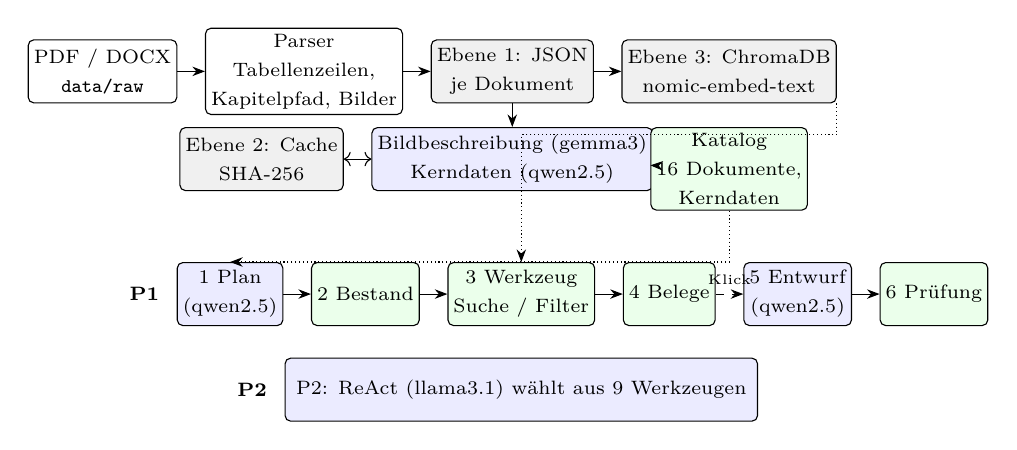
\begin{tikzpicture}[font=\scriptsize, node distance=3mm and 3.5mm,
    box/.style={draw, rounded corners=2pt, align=center, minimum height=8mm, inner sep=2pt},
    store/.style={box, fill=gray!12}, llmbox/.style={box, fill=blue!8}, codebox/.style={box, fill=green!8},
    arr/.style={-{Stealth[length=1.6mm]}}]
  \node[box] (raw) {PDF / DOCX\\\texttt{data/raw}};
  \node[box, right=of raw] (parse) {Parser\\Tabellenzeilen,\\Kapitelpfad, Bilder};
  \node[store, right=of parse] (json) {Ebene 1: JSON\\je Dokument};
  \node[llmbox, below=of json] (enrich) {Bildbeschreibung (gemma3)\\Kerndaten (qwen2.5)};
  \node[store, left=of enrich] (cache) {Ebene 2: Cache\\SHA-256};
  \node[store, right=of json] (chroma) {Ebene 3: ChromaDB\\nomic-embed-text};
  \node[codebox, below=of chroma] (cat) {Katalog\\16 Dokumente,\\Kerndaten};
  % P1
  \node[llmbox, below=9mm of cache, xshift=-4mm] (plan) {1 Plan\\(qwen2.5)};
  \node[codebox, right=of plan] (bestand) {2 Bestand};
  \node[codebox, right=of bestand] (tool) {3 Werkzeug\\Suche / Filter};
  \node[codebox, right=of tool] (bel) {4 Belege};
  \node[llmbox, right=of bel] (draft) {5 Entwurf\\(qwen2.5)};
  \node[codebox, right=of draft] (check) {6 Prüfung};
  \node[left=1mm of plan, font=\scriptsize\bfseries] {P1};
  \node[llmbox, below=4mm of tool, minimum width=6cm] (p2) {P2: ReAct (llama3.1) wählt aus 9 Werkzeugen};
  \node[left=1mm of p2, font=\scriptsize\bfseries] {P2};
  \draw[arr] (raw) -- (parse); \draw[arr] (parse) -- (json); \draw[arr] (json) -- (enrich);
  \draw[arr, <->] (enrich) -- (cache); \draw[arr] (json) -- (chroma); \draw[arr] (enrich) -- (cat);
  \draw[arr] (plan) -- (bestand); \draw[arr] (bestand) -- (tool); \draw[arr] (tool) -- (bel);
  \draw[arr, dashed] (bel) -- node[above, font=\tiny]{Klick} (draft); \draw[arr] (draft) -- (check);
  \draw[arr, densely dotted] (chroma.south east) |- ++(0,-4mm) -| (tool.north);
  \draw[arr, densely dotted] (cat.south) |- (plan.north);
\end{tikzpicture}
\caption{Architektur: Einlesen in drei Speicherebenen, darunter die sechs Stufen von P1 (grün: Code, blau: Sprachmodell) und P2}
\label{fig:architektur}
\end{figure}


\section{Text-RAG für Fließtext}
\label{sec:textrag}

Der Parser liest PDF mit PyMuPDF und DOCX mit python-docx. Statt nach fester Zeichenzahl zu schneiden, folgt er der Struktur. Überschriften erkennt er an der Schriftgröße (ab 1,25-fach) oder an Fettdruck (ab 1,05-fach). Jeder Block bekommt den Pfad seiner Überschriften mit, etwa \enquote{Stromliefervertrag > §\,3 Preise}. Absätze unter 20 Zeichen hängt er an den vorigen an, damit ein Betrag nicht allein steht, über 1\,500 Zeichen teilt er sie an Satzgrenzen. Aus 16 Dokumenten entstehen 436 Blöcke: 246 Text, 80 Überschriften, 108 Tabellenzeilen, 2 Bilder.

Vor dem Einbetten stelle ich jedem Block seinen Pfad voran, etwa \texttt{[Vertraege | Vertrag\_Wasser | §\,5 Vorauszahlung]}. Ohne ihn ist \enquote{210,00\,€ quartalsweise} irgendein Betrag, mit ihm gehört er zum Wasservertrag. ChromaDB liefert 20 Kandidaten nach Kosinus-Ähnlichkeit. Enthält der Pfad ein Wort der Frage, zählt der Score 1,5-fach, die besten fünf gehen weiter. Jeden Baustein kann ich einzeln abschalten und messen. Drei flogen so wieder raus (Tabelle~\ref{tab:ablation}): BM25 brachte nichts, weil der Pfad die Fachwörter schon enthält, ein Reranker verschlechterte die Reihenfolge, und Umformulieren der Frage durch ein Modell senkte den Anteil mit richtigem Dokument unter den ersten fünf von 100 auf 68\,\%. \emph{Schwäche:} Fußzeilen erkennt der Parser nicht immer. In der Stromrechnung landen Handelsregister und IBAN als \enquote{Tabellenzeile} im Index.

\section{Tabellen- und Bild-RAG}
\label{sec:tabbild}

Die meisten Werte stehen in Tabellen. Der Parser schneidet sie deshalb zuerst aus dem Fließtext und speichert jede Zeile als Block, in dem jeder Wert seinen Spaltenkopf behält:
\begin{center}\small
\texttt{Position: Arbeitspreis Strom | Menge: 3.400 kWh | Einzelpreis: 34,500 ct/kWh | Gesamt netto (€): 1.173,00}
\end{center}
So weiß das Modell, ob eine Zahl netto oder brutto ist. gemma3:4b fasst zusätzlich jede Tabelle in einem Satz zusammen, damit auch allgemeine Fragen sie finden. Bilder unter 100 Pixeln (Logos, Linien) überspringe ich, die übrigen beschreibt gemma3:4b als Vision-Modell. Der Prompt verlangt bei Diagrammen Achsen und \emph{alle} ablesbaren Werte. Aus dem Verbrauchsdiagramm wird so \enquote{Jan: 380\,kWh, \dots, Jul: 150\,kWh}, und erst dadurch ist die Frage nach dem Monat mit dem niedrigsten Verbrauch beantwortbar. \emph{Schwäche:} Es gibt nur zwei Bilder. Ob gemma unübersichtliche Diagramme richtig abliest, habe ich nicht systematisch getestet.

\section{Strukturierte Kerndaten statt SQL-Datenbank}
\label{sec:kerndaten}

Bei \enquote{Welche Verträge kann ich bis Jahresende kündigen?} muss ich \emph{alle} Verträge prüfen, da hilft Ähnlichkeitssuche nicht. Deshalb liest qwen2.5:7b beim Einlesen feste \emph{Kerndaten} aus, bei Rechnungen 11 Felder (Anbieter, Datum, Gesamtbetrag, Fälligkeit \dots), bei Verträgen 17 (Beginn, Laufzeitende, Kündigungsfrist, Abschlag \dots). Ollama erzwingt dabei ein JSON-Schema. Blind traue ich den Werten nicht: Steht ein Wert nicht wörtlich im Dokument, löscht Code ihn. In meiner ersten Version waren 49\,\% der Felder richtig, mit dieser Prüfung und getrennten Feldlisten sind es 96\,\%.

Aus den Kerndaten baut Code einen \emph{Katalog} mit einer Zeile je Dokument, etwa \enquote{[12] Vertrag · Volt \& Wärme AG · Heizstromvertrag WP-Natur}. Darauf laufen Filter wie \texttt{kuendigen\_bis <= 31.12.2026}. Das ist im Grunde ein SQL-\texttt{WHERE} in Python, eine echte Datenbank brauche ich bei 16 Dokumenten nicht. Kündigungstermine rechnet ein eigener Fristrechner aus Laufzeitende, Frist und Verlängerung, nie das Sprachmodell.

\paragraph{Warum kein GraphRAG?} Entitäten gäbe es genug: Personen, Anbieter, Verträge, Rechnungen, Zähler, Fahrzeuge. Relevante Beziehungen wären \enquote{Rechnung gehört zu Vertrag} oder \enquote{Vertrag läuft auf Person}. Ein Graph hilft bei Fragen über mehrere Dokumente (\enquote{Welche Rechnungen gehören zum Stromvertrag?}). Bei 16 Dokumenten ist aber jede dieser Kanten ein Vergleich zweier Kerndatenfelder (gleiche Vertragsnummer, gleicher Kunde), und das erledigen Katalog und Filter. Dazu kommen die Kosten: Ein Modell müsste alle 436 Blöcke auf Entitäten lesen, bei geschätzt 30\,s je Aufruf über drei Stunden, statt 16 Aufrufen für die Kerndaten. Meine erste Version hatte fünf Graph-Werkzeuge. Keine Testfrage brauchte sie, also habe ich sie entfernt.

\section{Der zentrale Orchestrator (P1) und der ReAct-Agent (P2)}
\label{sec:orchestrator}

P1 arbeitet in sechs festen Stufen, das Modell kommt nur zweimal vor:
\begin{enumerate}[nosep, leftmargin=*]
    \item \emph{Plan:} qwen2.5:7b füllt mit Frage und Katalog ein kleines JSON: Fragetyp (\texttt{wert}, \texttt{vergleich}, \texttt{frist}, \texttt{liste}, \texttt{fehlt}), Dokumentnummern, bei Listen einen Filter. Code prüft den Plan, etwa dass ein Vergleich Rechnung \emph{und} Vertrag enthält.
    \item \emph{Bestand:} Code prüft, ob es die Dokumentart gibt. Bei \enquote{private Haftpflichtversicherung} reicht nicht, dass \enquote{Haftpflicht} im Kfz-Schein steht, auch \enquote{privat} muss passen. Sonst kommt sofort \enquote{nicht belegt}.
    \item \emph{Werkzeug:} Werte sucht P1 nur in den geplanten Dokumenten, Listen filtert Python, Fristen rechnet der Fristrechner.
    \item \emph{Belege:} Die App zeigt die Treffer zuerst, nummeriert, nach Ordner, Datei und Kapitel geordnet und eingefärbt (grün ab 0,7, rot unter 0,4). Erst auf Klick schreibt das Modell.
    \item \emph{Entwurf:} qwen2.5:7b liefert JSON: jeden Wert mit Belegnummer, optional eine Rechnung wie \enquote{w2 $-$ w1} und einen Antwortsatz mit Platzhalter für das Ergebnis.
    \item \emph{Prüfung:} Code sucht jeden Wert in seinem Beleg, prüft netto/brutto und rechnet selbst. Bei Fehlern gibt es genau einen Korrekturversuch mit konkretem Hinweis (\enquote{14,00 steht nicht in Beleg~1}), danach fliegt Unbelegtes raus.
\end{enumerate}
P2 ist das Gegenmodell: llama3.1:8b überlegt nach dem ReAct-Muster, ruft eines von neun Werkzeugen auf (Suchen, Kerndaten, Listen, Filter, Rechner), liest das Ergebnis und entscheidet selbst weiter. Nach sechs Schritten oder 300\,s muss es antworten. Zahlprüfung und Quellen sind dieselben wie bei P1.

\paragraph{Eine Frage im Detail.} Testfrage T14 fragt, um wie viel die neue Wasser-Vorauszahlung ab Februar 2025 höher ist als im Vertrag. Der Plan wählt in 17\,s Rechnung und Vertrag, schnell, weil der Katalog im Prompt-Cache liegt und nur 23 neue Tokens gelesen werden. Die Suche liefert in 0,2\,s zwölf Belege, darunter 210,00\,€ (Vertrag) und \enquote{Ab dem 15.02.2025 \dots{} 225,00\,€} (Rechnung). Der Entwurf braucht 113\,s, davon 79\,s nur zum Einlesen von etwa 1\,500 Tokens Belegen, und antwortet richtig mit 15,00\,€. Im Protokoll habe ich aber gesehen, dass das Modell selbst gerechnet hat, statt den Platzhalter zu nutzen. Die Zahlprüfung ließ \enquote{15} nur durch, weil die Zahl zufällig als Tag im Datum 15.02.2025 steht.

\paragraph{Antwortzeit.} Mein Prozessor liest nur etwa 18 Tokens/s ein. Antworten mit Entwurf dauern deshalb rund 100\,s statt der angepeilten 60\,s, Listen und Ablehnungen 10 bis 20\,s. Dass in einer Messung sogar der Plan 100\,s brauchte, lag an meinem Messaufbau: Das Modell von P2 verdrängte das von P1 aus dem Speicher.

%!TEX root = ../../../main.tex

\chapter{Vorverarbeitung und Suche}
\label{chap:vorverarbeitung}

\paragraph{Einlesen.} Der Parser liest PDF mit PyMuPDF und DOCX mit python-docx. Zuerst sucht er Tabellen: Jede Zeile wird ein eigener Block \enquote{Spalte: Wert | Spalte: Wert}, so steht der Spaltenkopf bei jeder Zahl. Überschriften erkennt er an Schriftgröße (ab 1,25-fach) oder Fettdruck und führt einen Kapitelpfad mit. Absätze unter 20 Zeichen hängt er an den vorigen Block, über 1500 Zeichen teilt er an Satzgrenzen. Bilder beschreibt gemma3:4b mit allen ablesbaren Werten. Aus 16 Dokumenten entstehen 436 Blöcke.

\begin{lstlisting}[language={}, basicstyle=\ttfamily\scriptsize, caption={Eine Tabellenzeile im JSON-Zwischenformat (gekürzt)}, label=lst:chunk, frame=single, breaklines=true]
{"chunk_type": "table_row", "content": "Gebührenart: Schmutzwassergebühr (Kanal) | Menge / Bemessung: 125,0 m³ | Satz: 2,80 €/m³ | ... | Brutto (€): 416,50",
 "heading_stack": ["ZWECKVERBAND WASSERVERSORGUNG", "Abgabenbescheid: Wasser & Abwasser 2024", "2. Gebührenberechnung ..."],
 "page_number": 1, "metadata": {"filename": "Rechnung_Wasser_Zweckverband_2024.pdf", "folder": "Rechnungen", "reconstructed": true}}
\end{lstlisting}

\paragraph{Speicherebenen und Kerndaten.} Ebene~1 ist eine lesbare JSON-Datei je Dokument (Listing~\ref{lst:chunk}). Ebene~2 speichert teure Modellausgaben unter einem SHA-256-Schlüssel, damit eine Parser-Änderung keine neuen Modellaufrufe kostet. Ebene~3 ist ChromaDB. Zusätzlich füllt qwen2.5:7b je Dokument 19 Kerndatenfelder. Code löscht jeden Wert, der nicht im Dokumenttext steht. 96\,\% der Felder stimmen mit meinen Sollwerten überein.

\paragraph{Suche.} Beim Einbetten (nomic-embed-text) setze ich vor jeden Block seinen Pfad \texttt{[Ordner | Datei | Kapitel]}. So wird \enquote{2,80\,€/m³} als Teil der \emph{Wasserabrechnung} gespeichert und nicht als irgendeine Zahl. ChromaDB liefert 20 Kandidaten nach Kosinus-Ähnlichkeit (\texttt{base}). Passt ein Wort der Frage zu Ordner, Datei oder Kapitel, wird mit 1,5 multipliziert (\texttt{boost}), und die besten fünf gehen an den Prototyp. BM25, einen Reranker und das Umformulieren der Frage habe ich gemessen (Anhang~\ref{app:messungen}). Keiner war besser, also sind sie aus.

%!TEX root = ../../../main.tex

\chapter{Reverse Engineering: Habe ich verstanden, was gebaut wurde?}
\label{chap:reverse}

Den Code habe ich mit einem KI-Assistenten geschrieben. Damit ich trotzdem jedes Teil verstehe, bin ich nach jedem Meilenstein rückwärts vorgegangen. Ich habe nicht gefragt, was der Code tun soll, sondern nachgesehen, was er tut. Das geschah in drei Schritten. \emph{Erstens} steht in \texttt{docs/reverse\_engineering.md} für jede Datei, was hinein- und herausgeht, welche Bibliothek sie nutzt und welcher Test sie absichert. \emph{Zweitens} prüfen 104 Unit-Tests die Bausteine einzeln, etwa \enquote{eine neue Überschrift ersetzt die alte auf gleicher Ebene}. Dabei sperrt ein Test-Hook jeden Modellaufruf, sodass das Verhalten nachweislich aus dem Code kommt. \emph{Drittens} habe ich einzelne Fragen durch das ganze System verfolgt und jede Zwischendatei angesehen.

\paragraph{Eine Frage von Anfang bis Ende.} Frage T14 lautet: \enquote{Wurde die Schmutzwassergebühr in der Wasserabrechnung 2024 zu dem Satz berechnet, der im Wasservertrag steht?}
\begin{enumerate}[nosep, leftmargin=*]
    \item \emph{Parser:} PyMuPDF erkennt auf der Wasserrechnung nur die Kopfzeile der Tabelle. Der Parser baut die Zeilen aus den Wortpositionen nach (\texttt{"reconstructed": true}, Listing~\ref{lst:chunk}).
    \item \emph{Suche:} Die Zeile hat $\text{base}=0{,}77$. \enquote{Wasser} steht im Dateinamen, also $\text{boost}=1{,}5$ und $\text{final}=1{,}15$. Alle sechs Belege stammen aus der Rechnung, der Wasser\emph{vertrag} ist nicht dabei.
    \item \emph{Entwurf:} qwen2.5:7b liefert als JSON den Wert \enquote{2,80\,€/m³} aus Beleg~2, eine unnötige Rechnung \enquote{416,50} und die Antwort \enquote{Ja, \dots\ wie im Vertrag festgelegt [2]}.
    \item \emph{Prüfung und Zeit:} Code findet \enquote{2,80\,€/m³} in Beleg~2 und verwirft die unnötige Rechnung. Von 98\,s gehen 76\,s auf das Lesen des Prompts (1436 Tokens), 22\,s auf die Antwort.
\end{enumerate}
Daraus habe ich drei Dinge gelernt. Erstens kommt die Wartezeit vom langen Kontext, nicht von der Antwort. Zweitens stimmt die Zahl, aber \enquote{wie im Vertrag festgelegt} ist nicht belegt. Drittens sieht meine Zahlprüfung das nicht, weil sie nur Zahlen prüft. Deshalb nutze ich zusätzlich RAGAS-Faithfulness (Kapitel~\ref{chap:evaluation}).

\paragraph{Was dabei aufgefallen ist.} In der ersten Version (Version1) fand ich so Fehler, die kein Endergebnis verraten hätte. Der Parser stürzte bei allen PDF-Verträgen ab, weil eine Funktion in drei Fällen drei statt zwei Werte zurückgab. Der Kapitelpfad stapelte \enquote{§ 1 > § 2 > § 3}, statt § 1 durch § 2 zu ersetzen. Der Reranker lud beim Start ein Modell aus dem Internet, das System war also nicht offline. 15 Zusatzwerkzeuge, davon fünf für einen Wissensgraphen, waren nie gegen \enquote{ohne} gemessen worden; ich habe sie entfernt. Auch meine eigene Bewertung hatte einen Fehler: Sie las \enquote{wenn nicht gekündigt} als Verneinung und erkannte die neue Ablehnungsformel nicht. Version2 sah dadurch 11 bis 14 Prozentpunkte schlechter aus. Seitdem hat auch die Bewertung Tests.

%!TEX root = ../../../main.tex

\chapter{Test- und Evaluationsstrategie}
\label{chap:evaluation}

\paragraph{Testsätze (Leitfrage~6).} Die KPI-Suite (\texttt{src/eval}) bewertet vier Sätze mit denselben Regeln. Der \emph{Kernsatz} enthält die neun Pflichtfragen: fünf Standardfragen, zwei Grenzfälle (Vorauszahlung Wasser gegen Vertrag, Verträge mit Verlängerung um ein Jahr) und zwei Fragen ohne Beleg. Der \emph{Entwicklungssatz} (54 Fragen) ist der einzige, an dem ich Fehler analysiert und Einstellungen gewählt habe. Der \emph{synthetische Satz} (51 Fragen) entsteht per Vorlage aus den Sollwerten, ähnlich der Testset-Generierung von RAGAS \cite{es2024}. Der \emph{zurückgehaltene Satz} (20 Fragen, alle fünf Typen) war vor dem Umbau geschrieben und per SHA-256 versiegelt.

\paragraph{Bewertung.} Statt eines LLM-Richters wie in RAGAS \cite{es2024}, der lokal langsam und selbst unzuverlässig wäre, prüfe ich deterministisch gegen Sollwerte. Korrekt ist eine Antwort, wenn jeder Sollwert in einem nicht verneinten Satz steht. Als \emph{Halluzination} zählt eine unbelegte Zahl oder eine Antwort auf eine unbeantwortbare Frage. Die Maße folgen der Literatur: Zitation nach ALCE \cite{gao2023alce}, Recall@5 und \gls{MRR} nach \cite{manning2008}, Enthaltung nach \cite{wen2024}, Werkzeugwahl nach \cite{qin2024}, Effizienz und Robustheit nach HELM \cite{liang2023}. Jede der 23 KPIs hat in \texttt{kpis.py} eine Definition, einen Zielwert und eine Begründung. Die Intervalle sind Wilson- \cite{wilson1927} bzw.\ Bootstrap-Intervalle \cite{efron1993}. Jede Antwort wird mit Trajektorie als JSONL gespeichert, personenbezogene Daten maskiert. Version1 lief unverändert auf denselben Fragen (Tabelle~\ref{tab:kpis}).

% automatisch erzeugt von src/eval/latex.py
\begin{table}[tp]
\centering
\scriptsize
\setlength{\tabcolsep}{3pt}
\begin{tabularx}{\textwidth}{@{}l l Y Y Y Y@{}}
\toprule
\textbf{KPI} & \textbf{Ziel} & \textbf{V1 P1} & \textbf{V1 P2} & \textbf{V2 P1} & \textbf{V2 P2} \\
\midrule
\multicolumn{6}{@{}l}{\textit{Qualität}} \\
Korrektheit & $\geq$ 80 \% & 53\,\% [37--68] & 53\,\% [37--68] & 48\,\% [36--61] & 52\,\% [39--64] \\
Treue & $\geq$ 95 \% & 96\,\% [91--99] & 98\,\% [95--100] & 98\,\% [96--100] & 82\,\% [69--92] \\
Halluzinationsrate & $\leq$ 5 \% & 16\,\% [7--30] & 11\,\% [4--24] & 10\,\% [5--21] & 22\,\% [14--35] \\
Zitationsrate & $\geq$ 90 \% & 90\,\% [70--97] & 89\,\% [67--97] & 94\,\% [80--98] & 52\,\% [37--67] \\
Zitationspräzision & $\geq$ 85 \% & 65\,\% [43--82] & 67\,\% [44--84] & 88\,\% [73--95] & 52\,\% [37--67] \\
Enthaltung & $\geq$ 90 \% & 86\,\% [49--97] & 86\,\% [49--97] & 60\,\% [31--83] & 60\,\% [31--83] \\
Fehl-Enthaltung & $\leq$ 10 \% & 35\,\% [21--53] & 42\,\% [26--59] & 31\,\% [20--45] & 17\,\% [9--30] \\
Recall@5 & $\geq$ 90 \% & 40\,\% [26--56] & 40\,\% [26--56] & 85\,\% [76--93] & 85\,\% [76--93] \\
Precision@5 & $\geq$ 60 \% & 43\,\% [26--59] & 43\,\% [26--59] & 72\,\% [61--82] & 72\,\% [61--82] \\
MRR & $\geq$ 0,80 & 0,49 [0,33--0,65] & 0,49 [0,33--0,65] & 0,86 [0,77--0,95] & 0,86 [0,77--0,95] \\
Beleg@5 & $\geq$ 85 \% & 52\,\% [34--69] & 52\,\% [34--69] & 77\,\% [63--87] & 77\,\% [63--87] \\
Feldgenauigkeit der Extraktion & $\geq$ 95 \% & 49\,\% [41--58] & 49\,\% [41--58] & 96\,\% [91--98] & 96\,\% [91--98] \\
\multicolumn{6}{@{}l}{\textit{Agent}} \\
Tool-Selection-Accuracy & $\geq$ 85 \% & -- & 10\,\% [3--25] & -- & 75\,\% [61--85] \\
Schritte je Frage & $\leq$ 4 & 0,0 [0,0--0,0] & 0,7 [0,4--1,0] & 0,0 [0,0--0,0] & 1,3 [1,1--1,4] \\
\multicolumn{6}{@{}l}{\textit{Effizienz}} \\
Latenz p50 & $\leq$ 60 s & 105\,s [92--136] & 176\,s [64--292] & 28\,s [11--38] & 36\,s [30--57] \\
Latenz p95 & $\leq$ 180 s & 254\,s [173--1876] & 948\,s [550--2935] & 62\,s [50--76] & 134\,s [105--195] \\
Tokens/s & $\geq$ 5 & 4,2 [3,9--4,4] & 3,5 [3,3--3,7] & 5,5 [5,4--5,5] & 5,1 [5,0--5,2] \\
Spitzen-RAM & $\leq$ 12 GB & 8,2\,GB & 8,2\,GB & 6,6\,GB & 9,1\,GB \\
Ingest-Zeit je Dokument & $\leq$ 120 s & -- & -- & 154\,s [140--171] & 154\,s [140--171] \\
Rewriting-Latenz & $<$ 500 ms & 0\,ms [0--0] & 0\,ms [0--0] & 2776\,ms [2546--2919] & 2776\,ms [2546--2919] \\
\multicolumn{6}{@{}l}{\textit{Robustheit}} \\
Konsistenz bei Wiederholung & $\geq$ 90 \% & 100\,\% [70--100] & 100\,\% [70--100] & 100\,\% [88--100] & 100\,\% [88--100] \\
Fehlerquote & $\leq$ 2 \% & 0\,\% [0--9] & 0\,\% [0--9] & 0\,\% [0--6] & 0\,\% [0--6] \\
Ausfallquote & 0 \% & 0\,\% [0--9] & 0\,\% [0--9] & 0\,\% [0--6] & 0\,\% [0--6] \\
\bottomrule
\end{tabularx}
\caption{KPIs der Ausgangsmessung (Version1) und der Schlussmessung (Version2) auf denselben Fragen, Punktwert mit 95-\%-Intervall (Anteile: Wilson, Mittelwerte und Perzentile: Bootstrap)}
\label{tab:kpis}
\end{table}


\paragraph{Ergebnis.} Version2 beantwortet nicht messbar mehr Fragen richtig als Version1: 48\,\% (P1) und 52\,\% (P2) gegen 53\,\%. Messbar besser ist alles vor dem Sprachmodell: Recall@5 stieg von 40 auf 85\,\%, die MRR von 0,49 auf 0,86, die Feldgenauigkeit von 49 auf 96\,\%, die richtige Werkzeugwahl von 10 auf 75\,\%. Die Latenz im Median sank von 105 bzw.\ 176\,s auf 28 bzw.\ 36\,s. P1 halluziniert seltener (10 statt 16\,\%) und zitiert präziser (88 statt 65\,\%). Im Kernsatz löst P2 16 von 18 Antworten, im zurückgehaltenen Satz lösen beide Prototypen nur 14 von 40. Auf dem Entwicklungssatz erreicht P1 nach der Abstimmung 81\,\%, auf ungesehenen Fragen 35\,\%. Die Abstimmung hat also vor allem Formulierungen der bekannten Fragen gelernt.

\paragraph{P1 gegen P2.} P1 löst Tabellen- und Rechenfragen besser (12 gegen 4 von 18), weil es die Zeilen direkt im Kontext sieht. P2 liest sie über \texttt{search\_tables} falsch, etwa 8300 statt 5500\,kWh. Fristfragen löst P2 vollständig (12 von 12), weil \texttt{list\_contracts} sie berechnet. P1 löst davon nur 2 und lehnt bei 31\,\% der beantwortbaren Fragen ab. P2 halluziniert dafür häufiger (22\,\%): Nach einem Gas- oder Fernwärmevertrag gefragt, antwortet es mit dem Heizstromvertrag.

\paragraph{Weiche zwischen P1 und P2.} Eine feste Textregel schickt Fragen zu Fristen, Listen über mehrere Dokumente und Vergleiche an P2, alle übrigen an P1 (\texttt{router.py}, ohne Sprachmodell). Die Idee stammt aus der Fehleranalyse oben, also aus dem zurückgehaltenen Satz. Die Muster und die Annahmeregel R9 wurden nur auf dem Entwicklungssatz festgelegt. Dort brachte die Weiche nichts: 44 von 54 Antworten richtig, genau wie P1 allein. R9 verlangt nur Gleichstand, daher wurde sie übernommen und einmal auf Kern- und zurückgehaltenem Satz ausgewertet, aus den Antworten der Schlussmessung. Ergebnis: 59\,\% richtig (34 von 58) gegen 48 und 52\,\%. Gegenüber P1 sind das $+10$ Prozentpunkte mit Intervall $[0;\,+21]$, gegenüber P2 $+7$ mit $[-7;\,+22]$, also nicht gesichert. Die Halluzinationsrate liegt mit 17\,\% zwischen beiden, die Latenz im Median bei 38\,s. Weil der zurückgehaltene Satz damit zum dritten Mal gesehen wurde und die Idee aus ihm stammt, ist der Wert eher optimistisch.

\paragraph{Transparenz.} Die erste Schlussmessung zeigte zwei Fehler. Die Bewertung erkannte die Ablehnungsformel von Version2 nicht; korrigiert, wurden alle Läufe neu bewertet. Außerdem gab P1 in 30 von 58 Antworten nur eine Belegnummer aus. Ich habe den Prompt auf dem Entwicklungssatz korrigiert und P1 neu gemessen. Für P1 wurde der zurückgehaltene Satz damit zweimal verwendet. Beide Läufe liegen im Repository.

%!TEX root = ../../../main.tex

\chapter{Reflexion}
\label{chap:reflexion}

\paragraph{Trägt die Grundidee?} Teilweise. Datensouveränität ist auf einem Laptop ohne Grafikkarte erreichbar: Kein Dokument verlässt den Rechner, eine Antwort dauert im Median eine halbe bis knapp zwei Minuten. Alles vor und nach dem Sprachmodell wurde messbar besser. Dazu gehören Parser, Kerndaten, Suche, Fristberechnung, Quellenliste und Bewertung. Die Korrektheit bestimmt aber das 8B-Modell, das Belege liest und formuliert. Sie blieb bei rund der Hälfte.
\begin{enumerate}[nosep, leftmargin=*]
    \item \textbf{Die Suche war nicht der Engpass.} Recall@5 lag schon ohne Zusätze bei 100\,\%. Das Modell lehnt trotz Beleg ab oder liest die falsche Zeile.
    \item \textbf{Was Code entscheidet, stimmt.} Fristfragen löst P2 alle, weil Python rechnet; Rechnen gehört ins Werkzeug \cite{schick2023}. Prüft Code die abgelesenen Werte, sinken die Ablehnungen, die Korrektheit kaum.
    \item \textbf{Abstimmen heißt Überanpassen.} 81\,\% auf dem Entwicklungssatz, 35\,\% auf ungesehenen Fragen.
    \item \textbf{Auch die Bewertung braucht Tests.} Ein fehlendes Muster für die eigene Ablehnungsformel ließ Version2 um 11 bis 14 Prozentpunkte schlechter aussehen.
    \item \textbf{Mehr Autonomie ist nicht automatisch besser.} Eine Weiche nach Fragetyp wie in Adaptive-RAG \cite{jeong2024} lag auf neuen Fragen 10 Prozentpunkte unter P1 allein.
\end{enumerate}

\paragraph{Ausblick.} Listenfragen gehören als Filter über die Kerndaten in den Code.

\endgroup

\clearpage

% Bibilography

\cleardoublepage
\begin{spacing}{1.175}
    \printbibliography
\end{spacing}

% Glossar
\ifshowGlossary
    \cleardoublepage
    \printglossary[style=altlist,title=\glossaryPhrase]
    %!TEX root = ../main.tex

%
% To create glossary run the following command:
% makeglossaries main.acn && makeglossaries main.glo
%

% Abkürzungen (nur verwendete erscheinen im Abkürzungsverzeichnis)

\newacronym{API}{API}{Application Programming Interface}
\newacronym{BM25}{BM25}{Best Matching 25 (lexikalisches Ranking-Verfahren)}
\newacronym{CPU}{CPU}{Central Processing Unit}
\newacronym{CRAG}{CRAG}{Corrective Retrieval-Augmented Generation}
\newacronym{GPU}{GPU}{Graphics Processing Unit}
\newacronym{JSON}{JSON}{JavaScript Object Notation}
\newacronym{KI}{KI}{Künstliche Intelligenz}
\newacronym{LLM}{LLM}{Large Language Model}
\newacronym{MRR}{MRR}{Mean Reciprocal Rank}
\newacronym{OCR}{OCR}{Optical Character Recognition}
\newacronym{OOM}{OOM}{Out of Memory}
\newacronym{RAG}{RAG}{Retrieval-Augmented Generation}
\newacronym{RRF}{RRF}{Reciprocal Rank Fusion}

\else
    % no glossary
\fi

% Appendix
\clearpage

\begin{appendices}
    % \chapter{Test}


    \appendixtoc
    % \addtocontents{toc}{\protect\setcounter{tocdepth}{0}}
    % !TeX root =../main.tex

\chapter{Testfragen mit Begründung}
\label{app:testsatz}

\begin{table}[H]
    \centering\footnotesize\setstretch{1.05}
    \begin{tabularx}{\textwidth}{@{}l l Y Y@{}}
        \toprule
        \textbf{Nr.} & \textbf{Art} & \textbf{Frage (gekürzt)} & \textbf{Was sie prüft} \\
        \midrule
        K1 & Standard a & Gesamtbetrag der LuminaStyle-Rechnung & Tabelle im PDF \\
        K2 & Standard b & Mindestlaufzeit des ConnectNet-Vertrags & Textstelle im DOCX \\
        K3 & Standard a & Arbeitspreis Hochtarif im Heizstromvertrag & richtige von zwei ähnlichen Zeilen \\
        K4 & Standard b & Zahlungsziel der Arztrechnung & Datum im Fließtext \\
        K5 & Standard a & Monat mit dem niedrigsten Stromverbrauch 2025 & Wert nur im Diagramm \\
        K6 & Grenzfall c & Vorauszahlung Wasserrechnung gegen Vertrag & zwei Dokumente verknüpfen \\
        K7 & Grenzfall d & Verträge mit Verlängerung um ein Jahr & Liste über alle Verträge \\
        K8 & Negativ e & Grundsteuer laut Grundsteuerbescheid & Dokumentart fehlt ganz \\
        K9 & Negativ e & Kündigungsfrist Handyvertrag bei Vodafone & Falle: Handyvertrag gibt es, aber bei ConnectNet \\
        \bottomrule
    \end{tabularx}
    \caption{Die neun Pflichtfragen (Kernsatz) und was jede prüft}
    \label{tab:kern}
\end{table}


Alle 24 Fragen des dritten versiegelten Testsatzes (\texttt{src/eval/sets/heldout3.json}), geschrieben und per SHA-256 versiegelt, bevor die geprüfte Antwort gebaut wurde. Die Sollwerte stammen aus dem Rohtext der Dokumente. Ergebnis: \checkmark{} = richtig nach der Regel aus Abschnitt~\ref{sec:kpis}. Beide Wiederholungen ergaben dieselben Antworten.

\begin{table}[H]
    \centering\scriptsize
    \setlength{\tabcolsep}{3pt}
    \begin{tabularx}{\textwidth}{@{}l l p{5.2cm} Y c c c@{}}
        \toprule
        \textbf{Nr.} & \textbf{Typ} & \textbf{Frage (gekürzt)} & \textbf{Warum diese Frage} & \textbf{P1 alt} & \textbf{P1} & \textbf{P2} \\
        \midrule
        T01 & a & Umsatzsteuer der LuminaStyle-Rechnung & Wert in der Summenzeile unter der Tabelle, nicht in einer Position & \checkmark & \checkmark & -- \\
        T02 & a & Versicherungssteuer der NordStern-Beitragsrechnung & Steuer und Beitrag sind zwei ähnliche Beträge & \checkmark & \checkmark & -- \\
        T03 & a & Nachtstrom (NT) netto, Heizstrom 2024 & Hoch- und Niedertarif stehen in Nachbarzeilen & \checkmark & \checkmark & \checkmark \\
        T04 & a & Blutentnahme auf der Arztrechnung & kleine Position unter vielen & \checkmark & \checkmark & -- \\
        T05 & a & Räderwechsel netto, Werkstatt & Netto- statt Bruttospalte & \checkmark & \checkmark & -- \\
        T06 & a & zwei Ladekabel brutto inkl.\ 19\,\% & Rechnen: 25,04\,€ $\times$ 1,19 = 29,80\,€ & -- & \checkmark & -- \\
        T07 & b & erste Laufzeit des Heizstromvertrags & Textstelle im DOCX-Vertrag & -- & -- & \checkmark \\
        T08 & b & Zahlungsweise im Stromvertrag & Antwort ist ein Wort, keine Zahl & -- & -- & -- \\
        T09 & b & Rücksendefrist bei LuminaStyle & Kleingedrucktes einer Rechnung & \checkmark & \checkmark & -- \\
        T10 & b & Abschlussdatum des Heizstromvertrags & mehrere Daten im Vertrag (Abschluss, Beginn, Ende) & -- & -- & -- \\
        T11 & b & Kündigung ConnectNet nach Mindestlaufzeit & zwei Teile (\enquote{jederzeit}, \enquote{ein Monat}) & \checkmark & -- & -- \\
        T12 & c & Grundpreis Stromrechnung gleich Vertrag? & Vergleich Rechnung--Vertrag, Werte gleich & \checkmark & -- & -- \\
        T13 & c & Differenz StreamPulse netto zu Vertrag brutto & zwei Dokumente und Rechnen (24,98 $-$ 20,99) & -- & -- & -- \\
        T14 & c & Schmutzwassergebühr laut Vertrag berechnet? & Vergleich Rechnung--Vertrag (Kapitel~\ref{chap:reverse}) & \checkmark & \checkmark & -- \\
        T15 & c & Abschlussdatum des Vertrags zur Wasserrechnung & Weg über die Vertragsnummer & -- & -- & -- \\
        T16 & d & Verträge mit monatlichen Abschlägen & Wasser zahlt quartalsweise und muss fehlen & -- & \checkmark & -- \\
        T17 & d & Erstlaufzeit endet 2027 & Filter über ein Datumsfeld & -- & \checkmark & \checkmark \\
        T18 & d & 2025 abgeschlossene Verträge & Filter über das Abschlussdatum & -- & -- & -- \\
        T19 & d & Rechnungen über 500\,€ & Liste über Rechnungen mit Schwelle & -- & -- & -- \\
        T20 & d & jährlich bezahlte Verträge & Filter über den Zahlungsturnus & -- & \checkmark & -- \\
        T21 & e & Rundfunkbeitrag laut Bescheid & Dokumentart fehlt ganz & \checkmark & \checkmark & \checkmark \\
        T22 & e & Zeitungsabo pro Monat & es gibt ein Abo, aber ein anderes (Streaming) & \checkmark & \checkmark & \checkmark \\
        T23 & e & Kündigungsfrist Servicevertrag Auto \& Service Müller & Anbieter hat nur eine Rechnung, keinen Vertrag & \checkmark & \checkmark & \checkmark \\
        T24 & e & Jahresabrechnung Strom 2025 & es gibt 2024 und eine Verbrauchsübersicht 2025 & \checkmark & -- & \checkmark \\
        \midrule
        \multicolumn{4}{@{}l}{\textbf{richtig}} & 13/24 & 14/24 & 7/24 \\
        \bottomrule
    \end{tabularx}
    \caption{Dritter versiegelter Testsatz: Begründung und Ergebnis je Frage}
    \label{tab:testsatz}
\end{table}

\chapter{Messungen zur Auswahl von Suche und Modellen}
\label{app:messungen}

% Aus LocalLLM/src/eval/results/modellauswahl/modellauswahl.md übertragen
\begin{table}[H]
    \centering\footnotesize
    \begin{tabularx}{\textwidth}{@{}Xrrrrrr@{}}
        \toprule
        Modell & Tool-Call & Werkzeug & p50 & Tok./s & RAM & Felder \\
        \midrule
        qwen2.5:7b  & 12/14 & 9/14  & 7,1\,s & 5,8  & 5,5\,GB & 100\,\% \\
        llama3.1:8b & 14/14 & 12/14 & 8,2\,s & 5,1  & 6,3\,GB & 100\,\% \\
        llama3.2    & 13/14 & 10/14 & 3,3\,s & 10,5 & 3,1\,GB & 97\,\% \\
        \midrule
        \multicolumn{7}{@{}p{\linewidth}@{}}{Rewriting p95: llama3.2 3,2\,s, gemma3:4b 4,5\,s, qwen2.5:7b 6,3\,s (Ziel $<$ 500\,ms). Vision gemma3:4b: 14/14 Diagrammwerte.} \\
        \bottomrule
    \end{tabularx}
    \caption{Modellauswahl auf dem Testrechner (CPU, 16\,GB RAM). Tool-Call: natives Tool-Calling, Werkzeug: richtiges Werkzeug gewählt, Felder: Kerndaten-Extraktion}
    \label{tab:modelle}
\end{table}


\begin{table}[H]
    \centering\small
    \begin{tabular}{lrrr}
        \toprule
        Variante & Recall@5 & MRR & Suche p50 \\
        \midrule
        ohne Boost & 100\,\% & 0,93 & 57\,ms \\
        Boost 1,5 (gewählt) & 100\,\% & 0,94 & 57\,ms \\
        + BM25 & 98\,\% & 0,95 & 62\,ms \\
        + Reranker & 99\,\% & 0,89 & 1088\,ms \\
        + Umformulieren durch Regeln & 99\,\% & 0,95 & 49\,ms \\
        + Umformulieren durch ein Modell & 68\,\% & 0,56 & 2546\,ms \\
        \bottomrule
    \end{tabular}
    \caption{Zusätze zur Suche auf 93 Entwicklungsfragen. Recall@5: richtiges Dokument unter den ersten fünf; MRR: mittlerer Kehrwert des Rangs des ersten richtigen Treffers}
    \label{tab:ablation}
\end{table}

    % \addtocontents{toc}{\protect\setcounter{tocdepth}{1}}
\end{appendices}
\end{document}
